\documentclass[../main/main.tex]{subfiles}

\begin{document}

\onlyinsubfile{%

}

% ==================================================================
% Section : 
% ==================================================================
\section{Section 2}%

\begin{frame}{Section 2 - Outline}
    \tableofcontents[currentsection, hideothersubsections]
\end{frame}


% ==================================================================
\subsection{Table}%

\begin{frame}{table}
    \begin{tabular}{| c | c |}
        \hline
        Spécifications                      & Fonction de transfert                    \\ \hline
        Suivi de trajectoires de références & $S(s) = T_{c \rightarrow \epsilon}$      \\ \hline
        Rejet de perturbation               & $G(s) S(s) = T_{p \rightarrow \epsilon}$ \\ \hline
        Atténuation des bruits              & $T(s) = T_{w \rightarrow \epsilon}$      \\ \hline
        Limitation de commande              & $K(s) S(s) = T_{c \rightarrow u}$        \\ \hline
    \end{tabular}
\end{frame}

% ==================================================================
\subsection{Tikz graphic}%

\begin{frame}{Tikz graphic}
    \begin{columns}[c]
        \begin{column}{0.6\textwidth}
            \centering
            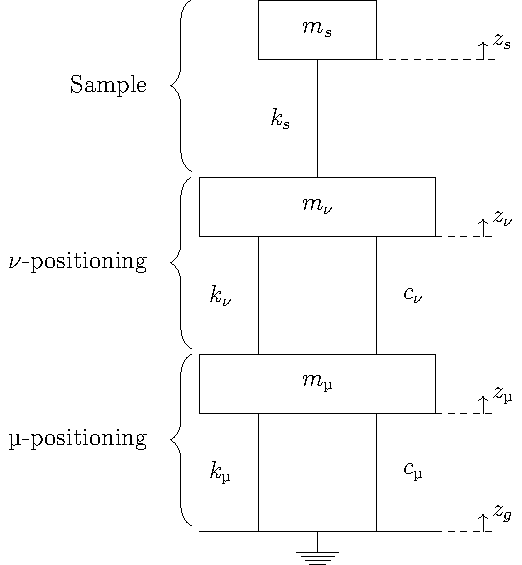
\includegraphics[width=1.0\textwidth, height=0.9\textheight, keepaspectratio]{mechanical}
        \end{column}
        \begin{column}{0.4\textwidth}
            \centering
            \begin{itemize}
                \item item1
                \item item2
            \end{itemize}
        \end{column}
    \end{columns}
\end{frame}

\end{document}

